% !TEX encoding = UTF-8 Unicode
\documentclass[a4paper]{report}
\usepackage{tikz}
\usepackage[margin=2.5cm]{geometry}
\usepackage{hyperref}
\usepackage{graphicx}
\usepackage{parskip}
\graphicspath{{figures/}{anotherFigureDirectory/}}
\graphicspath{ {./images/} }
\usepackage{listings}
\usepackage{wrapfig}
\usepackage{float}
\usepackage{color}
\usepackage[school,simplified]{pgf-umlcd}
\definecolor{bluekeywords}{rgb}{0.13,0.13,1}
\definecolor{greencomments}{rgb}{0,0.5,0}
\definecolor{turqusnumbers}{rgb}{0.17,0.57,0.69}
\definecolor{redstrings}{rgb}{0.5,0,0}
\definecolor{gray}{rgb}{0.13,0.13,0.13}
\lstdefinelanguage{FSharp}
                {morekeywords={let, new, match, with, rec, open, module,
                namespace, type, of, member, and, for, in, do, begin, end, fun,
                function, try, mutable, if, then, else},
                keywordstyle=\color{bluekeywords},
                sensitive=false,
                numbers=left,  % where to put the line-numbers;(none, left, right)
                numberstyle=\tiny\color{gray},
                morecomment=[l][\color{greencomments}]{///},
                morecomment=[l][\color{greencomments}]{//},
                morecomment=[s][\color{greencomments}]{{(*}{*)}},
                morestring=[b]",
                showstringspaces=false,
                stringstyle=\color{redstrings}
                }

\title{PoP - Ugeopgave 11}
\author{Christoffer, Inge og Pernille}
\date{\today}

\begin{document}
\maketitle
\tikzstyle{block} = [rectangle, draw, fill=blue!20, text centered,
    rounded corners, minimum height=2.5em]
\tikzstyle{cloud} = [rectangle, draw, fill=white, text centered,
    rounded corners, minimum height = 2em]
\tikzstyle{line} = [draw, -latex]


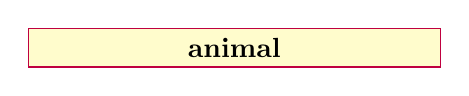
\begin{tikzpicture}
 \begin{class}[text width=5cm]{animal}{0,0}
 \end{class}
\end{tikzpicture}

Opgaven:
Uppercase er det ene hold lowercase er modstander.
Vi skal ikke foreslå felter, som en modstander brik kan rykke hen på. 
Hver opmærksom på brikkers mulighed for at rykke forbi hinanden.

Available moves skal tage højde for, hvilken type modstander brik, der er indenfor rækkevidde, da det afgører, hvor det skal være muligt og ikke-muligt at rykke hen på. 

I bordet laves et array i 2d, hvor i hvert coordinat er der some eller none brik.
Husk at pakke option typen ud, før den kan "bruges" i andet kode som værende brik.

Vi skal lave noget kode, der kan tilgå alle brikker på bordet.

er det en konge der rykkes skal der tjekkes for alle vertikale og horisontale squares der er til bordets yderkanter, for om der står et tårn, da et tårn potentielt ved næste tur kan rykke hele board-bredden og højden. Det kan vi dog ikke tjekke via tårnets possibleMoves, fordi den givne kode er sat til, at et tårn ikke kan rykke sig forbi en anden brik og derfor ikke medtager pladserne på modsatte side af en modstanden ud til bordets kant.

\end{document}